% Options for packages loaded elsewhere
\PassOptionsToPackage{unicode}{hyperref}
\PassOptionsToPackage{hyphens}{url}
\PassOptionsToPackage{dvipsnames,svgnames,x11names}{xcolor}
%
\documentclass[
]{article}
\usepackage{amsmath,amssymb}
\usepackage{iftex}
\ifPDFTeX
  \usepackage[T1]{fontenc}
  \usepackage[utf8]{inputenc}
  \usepackage{textcomp} % provide euro and other symbols
\else % if luatex or xetex
  \usepackage{unicode-math} % this also loads fontspec
  \defaultfontfeatures{Scale=MatchLowercase}
  \defaultfontfeatures[\rmfamily]{Ligatures=TeX,Scale=1}
\fi
\usepackage{lmodern}
\ifPDFTeX\else
  % xetex/luatex font selection
\fi
% Use upquote if available, for straight quotes in verbatim environments
\IfFileExists{upquote.sty}{\usepackage{upquote}}{}
\IfFileExists{microtype.sty}{% use microtype if available
  \usepackage[]{microtype}
  \UseMicrotypeSet[protrusion]{basicmath} % disable protrusion for tt fonts
}{}
\makeatletter
\@ifundefined{KOMAClassName}{% if non-KOMA class
  \IfFileExists{parskip.sty}{%
    \usepackage{parskip}
  }{% else
    \setlength{\parindent}{0pt}
    \setlength{\parskip}{6pt plus 2pt minus 1pt}}
}{% if KOMA class
  \KOMAoptions{parskip=half}}
\makeatother
\usepackage{xcolor}
\usepackage[margin=1in]{geometry}
\usepackage{color}
\usepackage{fancyvrb}
\newcommand{\VerbBar}{|}
\newcommand{\VERB}{\Verb[commandchars=\\\{\}]}
\DefineVerbatimEnvironment{Highlighting}{Verbatim}{commandchars=\\\{\}}
% Add ',fontsize=\small' for more characters per line
\usepackage{framed}
\definecolor{shadecolor}{RGB}{248,248,248}
\newenvironment{Shaded}{\begin{snugshade}}{\end{snugshade}}
\newcommand{\AlertTok}[1]{\textcolor[rgb]{0.94,0.16,0.16}{#1}}
\newcommand{\AnnotationTok}[1]{\textcolor[rgb]{0.56,0.35,0.01}{\textbf{\textit{#1}}}}
\newcommand{\AttributeTok}[1]{\textcolor[rgb]{0.13,0.29,0.53}{#1}}
\newcommand{\BaseNTok}[1]{\textcolor[rgb]{0.00,0.00,0.81}{#1}}
\newcommand{\BuiltInTok}[1]{#1}
\newcommand{\CharTok}[1]{\textcolor[rgb]{0.31,0.60,0.02}{#1}}
\newcommand{\CommentTok}[1]{\textcolor[rgb]{0.56,0.35,0.01}{\textit{#1}}}
\newcommand{\CommentVarTok}[1]{\textcolor[rgb]{0.56,0.35,0.01}{\textbf{\textit{#1}}}}
\newcommand{\ConstantTok}[1]{\textcolor[rgb]{0.56,0.35,0.01}{#1}}
\newcommand{\ControlFlowTok}[1]{\textcolor[rgb]{0.13,0.29,0.53}{\textbf{#1}}}
\newcommand{\DataTypeTok}[1]{\textcolor[rgb]{0.13,0.29,0.53}{#1}}
\newcommand{\DecValTok}[1]{\textcolor[rgb]{0.00,0.00,0.81}{#1}}
\newcommand{\DocumentationTok}[1]{\textcolor[rgb]{0.56,0.35,0.01}{\textbf{\textit{#1}}}}
\newcommand{\ErrorTok}[1]{\textcolor[rgb]{0.64,0.00,0.00}{\textbf{#1}}}
\newcommand{\ExtensionTok}[1]{#1}
\newcommand{\FloatTok}[1]{\textcolor[rgb]{0.00,0.00,0.81}{#1}}
\newcommand{\FunctionTok}[1]{\textcolor[rgb]{0.13,0.29,0.53}{\textbf{#1}}}
\newcommand{\ImportTok}[1]{#1}
\newcommand{\InformationTok}[1]{\textcolor[rgb]{0.56,0.35,0.01}{\textbf{\textit{#1}}}}
\newcommand{\KeywordTok}[1]{\textcolor[rgb]{0.13,0.29,0.53}{\textbf{#1}}}
\newcommand{\NormalTok}[1]{#1}
\newcommand{\OperatorTok}[1]{\textcolor[rgb]{0.81,0.36,0.00}{\textbf{#1}}}
\newcommand{\OtherTok}[1]{\textcolor[rgb]{0.56,0.35,0.01}{#1}}
\newcommand{\PreprocessorTok}[1]{\textcolor[rgb]{0.56,0.35,0.01}{\textit{#1}}}
\newcommand{\RegionMarkerTok}[1]{#1}
\newcommand{\SpecialCharTok}[1]{\textcolor[rgb]{0.81,0.36,0.00}{\textbf{#1}}}
\newcommand{\SpecialStringTok}[1]{\textcolor[rgb]{0.31,0.60,0.02}{#1}}
\newcommand{\StringTok}[1]{\textcolor[rgb]{0.31,0.60,0.02}{#1}}
\newcommand{\VariableTok}[1]{\textcolor[rgb]{0.00,0.00,0.00}{#1}}
\newcommand{\VerbatimStringTok}[1]{\textcolor[rgb]{0.31,0.60,0.02}{#1}}
\newcommand{\WarningTok}[1]{\textcolor[rgb]{0.56,0.35,0.01}{\textbf{\textit{#1}}}}
\usepackage{graphicx}
\makeatletter
\def\maxwidth{\ifdim\Gin@nat@width>\linewidth\linewidth\else\Gin@nat@width\fi}
\def\maxheight{\ifdim\Gin@nat@height>\textheight\textheight\else\Gin@nat@height\fi}
\makeatother
% Scale images if necessary, so that they will not overflow the page
% margins by default, and it is still possible to overwrite the defaults
% using explicit options in \includegraphics[width, height, ...]{}
\setkeys{Gin}{width=\maxwidth,height=\maxheight,keepaspectratio}
% Set default figure placement to htbp
\makeatletter
\def\fps@figure{htbp}
\makeatother
\setlength{\emergencystretch}{3em} % prevent overfull lines
\providecommand{\tightlist}{%
  \setlength{\itemsep}{0pt}\setlength{\parskip}{0pt}}
\setcounter{secnumdepth}{-\maxdimen} % remove section numbering
\ifLuaTeX
  \usepackage{selnolig}  % disable illegal ligatures
\fi
\IfFileExists{bookmark.sty}{\usepackage{bookmark}}{\usepackage{hyperref}}
\IfFileExists{xurl.sty}{\usepackage{xurl}}{} % add URL line breaks if available
\urlstyle{same}
\hypersetup{
  colorlinks=true,
  linkcolor={Maroon},
  filecolor={Maroon},
  citecolor={Blue},
  urlcolor={blue},
  pdfcreator={LaTeX via pandoc}}

\author{}
\date{\vspace{-2.5em}}

\begin{document}

\begin{Shaded}
\begin{Highlighting}[]
\CommentTok{\# Loading the data set}
\NormalTok{games }\OtherTok{\textless{}{-}} \FunctionTok{read.csv}\NormalTok{(}\StringTok{\textquotesingle{}data/games\_clean.csv\textquotesingle{}}\NormalTok{)}
\end{Highlighting}
\end{Shaded}

\begin{Shaded}
\begin{Highlighting}[]
\CommentTok{\# Checking the structure of the dataset}
\FunctionTok{str}\NormalTok{(games)}
\end{Highlighting}
\end{Shaded}

\begin{verbatim}
## 'data.frame':    75404 obs. of  59 variables:
##  $ AppID                              : int  20200 655370 1732930 1355720 1139950 1469160 1659180 1968760 1178150 320150 ...
##  $ Name                               : chr  "Galactic Bowling" "Train Bandit" "Jolt Project" "Henosis™" ...
##  $ Release.date                       : chr  "2008-10-21" "2017-10-12" "2021-11-17" "2020-07-23" ...
##  $ Peak.CCU                           : int  NA NA NA NA NA 68 3 2 1 NA ...
##  $ Required.age                       : int  0 0 0 0 0 0 0 0 0 0 ...
##  $ Price                              : num  19.99 0.99 4.99 5.99 0 ...
##  $ DLC.count                          : int  0 0 0 0 0 0 1 0 0 0 ...
##  $ Windows                            : int  1 1 1 1 1 1 1 1 1 1 ...
##  $ Mac                                : int  0 1 0 1 1 0 0 0 0 1 ...
##  $ Linux                              : int  0 0 0 1 0 0 0 0 0 1 ...
##  $ Metacritic.score                   : int  NA NA NA NA NA NA NA NA NA NA ...
##  $ User.score                         : int  NA NA NA NA NA NA NA NA NA NA ...
##  $ Positive                           : int  6 53 NA 3 50 87 21 NA 76 225 ...
##  $ Negative                           : int  11 5 NA NA 8 49 7 NA 6 45 ...
##  $ Score.rank                         : int  NA NA NA NA NA NA NA NA NA NA ...
##  $ Achievements                       : int  30 12 0 0 17 0 62 0 25 32 ...
##  $ Recommendations                    : int  0 0 0 0 0 0 0 0 0 0 ...
##  $ Average.playtime.forever           : int  NA NA NA NA NA NA NA NA NA 703 ...
##  $ Average.playtime.two.weeks         : int  NA NA NA NA NA NA NA NA NA NA ...
##  $ Median.playtime.forever            : int  NA NA NA NA NA NA NA NA NA 782 ...
##  $ Median.playtime.two.weeks          : int  NA NA NA NA NA NA NA NA NA NA ...
##  $ Publishers                         : chr  "Perpetual FX Creative" "Wild Rooster" "Campião Games" "Odd Critter Games" ...
##  $ Categories                         : chr  "Single-player,Multi-player,Steam Achievements,Partial Controller Support" "Single-player,Steam Achievements,Full controller support,Steam Leaderboards,Remote Play on Phone,Remote Play on"| __truncated__ "Single-player" "Single-player,Full controller support" ...
##  $ Genres                             : chr  "Casual,Indie,Sports" "Action,Indie" "Action,Adventure,Indie,Strategy" "Adventure,Casual,Indie" ...
##  $ Tags                               : chr  "Indie,Casual,Sports,Bowling" "Indie,Action,Pixel Graphics,2D,Retro,Arcade,Score Attack,Minimalist,Comedy,Singleplayer,Fast-Paced,Casual,Funny"| __truncated__ "" "2D Platformer,Atmospheric,Surreal,Mystery,Puzzle,Survival,Adventure,Linear,Singleplayer,Experimental,Platformer"| __truncated__ ...
##  $ Owners.min                         : num  0 0 0 0 0 50000 0 0 0 50000 ...
##  $ Owners.max                         : num  2e+04 2e+04 2e+04 2e+04 2e+04 1e+05 2e+04 2e+04 2e+04 1e+05 ...
##  $ Owners.mean                        : num  10000 10000 10000 10000 10000 75000 10000 10000 10000 75000 ...
##  $ Revenue                            : num  199900 9900 49900 59900 0 ...
##  $ Revenue.log                        : num  12.2 9.2 10.8 11 NA ...
##  $ Peak.CCU.log                       : num  NA NA NA NA NA ...
##  $ Positive.log                       : num  1.79 3.97 NA 1.1 3.91 ...
##  $ Negative.log                       : num  2.4 1.61 NA NA 2.08 ...
##  $ Lang.count                         : int  1 10 2 11 2 1 3 2 10 9 ...
##  $ Lang.English                       : int  1 1 1 1 1 1 1 1 1 1 ...
##  $ Lang.Spanish                       : int  0 1 0 1 1 0 0 0 1 1 ...
##  $ Lang.Chinese                       : int  0 1 0 1 0 0 0 0 1 0 ...
##  $ Lang.Russian                       : int  0 1 0 1 0 0 1 0 1 1 ...
##  $ Lang.German                        : int  0 1 0 1 0 0 0 1 1 1 ...
##  $ Lang.Portuguese                    : int  0 1 1 1 0 0 0 0 0 1 ...
##  $ Lang.French                        : int  0 1 0 1 0 0 0 0 1 1 ...
##  $ Lang.Italian                       : int  0 1 0 1 0 0 0 0 1 1 ...
##  $ Publishers.count                   : int  1 4 1 1 1 1 2 35 26 3 ...
##  $ Genre.Indie                        : int  1 1 1 1 1 0 1 0 0 1 ...
##  $ Genre.Casual                       : int  1 0 0 1 0 1 0 1 0 0 ...
##  $ Genre.Action                       : int  0 1 1 0 0 0 0 0 0 1 ...
##  $ Genre.Adventure                    : int  0 0 1 1 1 1 0 0 1 1 ...
##  $ Genre.Simulation                   : int  0 0 0 0 0 0 0 0 1 0 ...
##  $ Genre.Strategy                     : int  0 0 1 0 0 1 1 0 1 0 ...
##  $ Category.Single.player             : int  1 1 1 1 1 1 1 1 1 1 ...
##  $ Category.Steam.Achievements        : int  1 1 0 0 1 0 1 0 1 1 ...
##  $ Category.Steam.Cloud               : int  0 0 0 0 0 0 1 1 0 1 ...
##  $ Category.Full.controller.support   : int  0 1 0 1 0 0 0 0 1 0 ...
##  $ Category.Multi.player              : int  1 0 0 0 0 1 0 0 0 0 ...
##  $ Category.Partial.Controller.Support: int  1 0 0 0 0 0 0 0 0 1 ...
##  $ Category.Steam.Trading.Cards       : int  0 0 0 0 0 0 0 0 0 1 ...
##  $ Category.PvP                       : int  0 0 0 0 0 1 0 0 0 0 ...
##  $ Category.Co.op                     : int  0 0 0 0 0 1 0 0 0 0 ...
##  $ Category.Online.PvP                : int  0 0 0 0 0 1 0 0 0 0 ...
\end{verbatim}

\hypertarget{linear-model}{%
\section{Linear model}\label{linear-model}}

A Linear Model is a statistical method used to model the relationship
between a dependent (target) variable and one or more independent
variables. The basic idea of a linear model is to represent the
dependent variable as a linear combination of the independent variables.
Linear models can be extended to consider multiple independent variables
and then it is called multiple linear model.

A linear regression model typically utilizes count and continuous data.
For binary data, more suitable models are available. Below, the data
types are briefly described:

\begin{itemize}
\tightlist
\item
  Binary Data: Consists of values such as `True' / `False' or `1' / `0'.
  An example of binary data is whether a certain programming language is
  supported or not.
\item
  Count Data: Comprises integer values (0, 1, 2, 3, \ldots) that
  represent the number of occurrences of something. For instance, the
  number of downloadable content (DLC) packs a game has can be
  categorized as count data.
\item
  Continuous Data: Encompasses any value within a given range. An
  example of continuous data is the amount of time a person has spent
  playing a particular game.
\end{itemize}

There are possible questions, which we can have a look at it with the
linear model:

\begin{itemize}
\tightlist
\item
  What factors influence the Peak Concurrent Users (CCU) of games on
  Steam?
\item
  What factors contribute to the financial success of a game, as
  measured by its revenue?
\end{itemize}

\hypertarget{peak-concurrent-users-ccu}{%
\subsection{Peak Concurrent Users
(CCU)}\label{peak-concurrent-users-ccu}}

Peak Concurrent Users (CCU) is a critical metric for gauging a game's
popularity, reflecting the highest number of players online at the same
time. It's an essential indicator for assessing a game's appeal and
success. Understanding CCU helps identify what drives player engagement
in the competitive gaming landscape.

\hypertarget{simple-model}{%
\subsubsection{Simple Model}\label{simple-model}}

First we start with a simple model and take only one predictor and start
with the variable revenue. We wanna predict if the revenue increases
with a higher Peak CCU.

\begin{Shaded}
\begin{Highlighting}[]
\NormalTok{df }\OtherTok{\textless{}{-}}\NormalTok{ games[, }\FunctionTok{c}\NormalTok{(}\StringTok{"Peak.CCU.log"}\NormalTok{, }\StringTok{"Revenue.log"}\NormalTok{)]}

\CommentTok{\# Creating a simple linear model}
\NormalTok{m }\OtherTok{\textless{}{-}} \FunctionTok{lm}\NormalTok{(Peak.CCU.log }\SpecialCharTok{\textasciitilde{}}\NormalTok{ Revenue.log, }\AttributeTok{data =}\NormalTok{ df)}

\CommentTok{\# Plot}
\FunctionTok{plot}\NormalTok{(df}\SpecialCharTok{$}\NormalTok{Revenue.log, df}\SpecialCharTok{$}\NormalTok{Peak.CCU.log, }\AttributeTok{pch =} \DecValTok{20}\NormalTok{, }\AttributeTok{col =} \StringTok{\textquotesingle{}lightblue\textquotesingle{}}\NormalTok{,}
     \AttributeTok{xlab =} \StringTok{"Revenue.log"}\NormalTok{, }\AttributeTok{ylab =} \StringTok{"Peak.CCU.log"}\NormalTok{)}

\CommentTok{\# Regression line}
\FunctionTok{abline}\NormalTok{(m, }\AttributeTok{col =} \StringTok{\textquotesingle{}blue\textquotesingle{}}\NormalTok{, }\AttributeTok{lwd =} \DecValTok{2}\NormalTok{)  }
\end{Highlighting}
\end{Shaded}

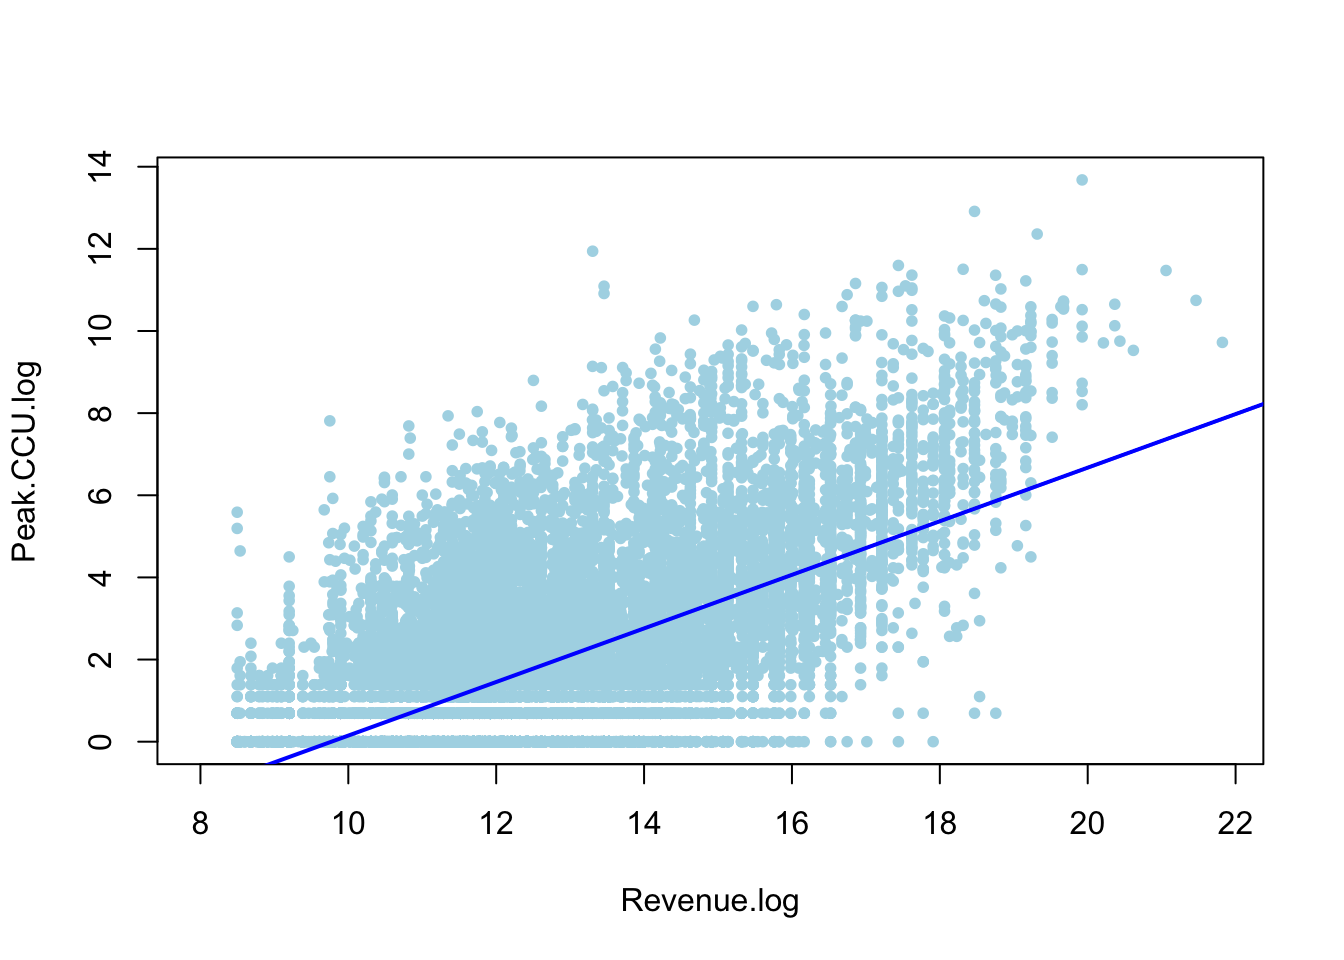
\includegraphics{Linear_model_files/figure-latex/simple lm ccu-1.pdf}

\begin{Shaded}
\begin{Highlighting}[]
\FunctionTok{summary}\NormalTok{(m)}
\end{Highlighting}
\end{Shaded}

\begin{verbatim}
## 
## Call:
## lm(formula = Peak.CCU.log ~ Revenue.log, data = df)
## 
## Residuals:
##     Min      1Q  Median      3Q     Max 
## -5.3104 -1.1356 -0.2795  0.7968  9.6376 
## 
## Coefficients:
##              Estimate Std. Error t value Pr(>|t|)    
## (Intercept) -6.376404   0.075354  -84.62   <2e-16 ***
## Revenue.log  0.652542   0.005905  110.51   <2e-16 ***
## ---
## Signif. codes:  0 '***' 0.001 '**' 0.01 '*' 0.05 '.' 0.1 ' ' 1
## 
## Residual standard error: 1.632 on 19032 degrees of freedom
##   (56370 observations deleted due to missingness)
## Multiple R-squared:  0.3909, Adjusted R-squared:  0.3909 
## F-statistic: 1.221e+04 on 1 and 19032 DF,  p-value: < 2.2e-16
\end{verbatim}

\begin{Shaded}
\begin{Highlighting}[]
\CommentTok{\# Creating a linear model for Peak Concurrent Users (CCU)}
\NormalTok{model }\OtherTok{\textless{}{-}} \FunctionTok{lm}\NormalTok{(Peak.CCU.log }\SpecialCharTok{\textasciitilde{}}\NormalTok{ Owners.mean }\SpecialCharTok{+}\NormalTok{ Metacritic.score }\SpecialCharTok{+}\NormalTok{ Positive.log }\SpecialCharTok{+} 
\NormalTok{              Publishers.count }\SpecialCharTok{+}\NormalTok{ Category.PvP }\SpecialCharTok{+}\NormalTok{ Recommendations }\SpecialCharTok{+}
\NormalTok{              Revenue.log, }\AttributeTok{data =}\NormalTok{ games)}

\CommentTok{\# Displaying the model summary}
\FunctionTok{summary}\NormalTok{(model)}
\end{Highlighting}
\end{Shaded}

\begin{verbatim}
## 
## Call:
## lm(formula = Peak.CCU.log ~ Owners.mean + Metacritic.score + 
##     Positive.log + Publishers.count + Category.PvP + Recommendations + 
##     Revenue.log, data = games)
## 
## Residuals:
##     Min      1Q  Median      3Q     Max 
## -6.3768 -0.8761 -0.0925  0.7655  7.1160 
## 
## Coefficients:
##                    Estimate Std. Error t value Pr(>|t|)    
## (Intercept)      -8.227e+00  3.085e-01 -26.663  < 2e-16 ***
## Owners.mean      -3.293e-08  1.552e-08  -2.122   0.0339 *  
## Metacritic.score  2.605e-02  2.851e-03   9.138  < 2e-16 ***
## Positive.log      6.682e-01  2.861e-02  23.353  < 2e-16 ***
## Publishers.count  3.668e-03  5.369e-04   6.832 1.02e-11 ***
## Category.PvP      5.603e-01  7.335e-02   7.638 3.01e-14 ***
## Recommendations   8.072e-06  1.055e-06   7.650 2.75e-14 ***
## Revenue.log       2.723e-01  2.751e-02   9.899  < 2e-16 ***
## ---
## Signif. codes:  0 '***' 0.001 '**' 0.01 '*' 0.05 '.' 0.1 ' ' 1
## 
## Residual standard error: 1.335 on 2807 degrees of freedom
##   (72589 observations deleted due to missingness)
## Multiple R-squared:  0.6956, Adjusted R-squared:  0.6949 
## F-statistic: 916.4 on 7 and 2807 DF,  p-value: < 2.2e-16
\end{verbatim}

\hypertarget{interpretation}{%
\subsubsection{Interpretation}\label{interpretation}}

This linear regression analysis reveals key factors driving the
popularity of video games, as indicated by peak concurrent users.
Notably, the model highlights several significant predictors of a game's
success. High Metacritic scores, positive user reviews, a diverse range
of publishers, player versus player (PvP) features, and strong
recommendations are all positively correlated with higher peak
concurrent users. Interestingly, more widely owned games show a slight
negative impact on peak CCU, possibly reflecting market saturation.

From an investment perspective, the analysis underscores the importance
of critical acclaim, positive user reception, and PvP elements in
driving a game's popularity. The strong statistical significance of
these factors suggests they are reliable indicators of a game's
potential success. With about 70\% of the variance in peak CCU explained
by these variables, investors can make more informed decisions on which
games or gaming companies to back. This model offers a valuable tool for
understanding the dynamics of the gaming market and identifying
promising investment opportunities.

\hypertarget{revenue}{%
\subsection{Revenue}\label{revenue}}

Revenue, indicating a game's financial success, hinges on factors like
price and sales volume. Higher-priced games can earn more, but the
number of players buying the game is crucial. DLC (Downloadable Content)
enhances appeal and can boost sales. Positive reviews and player
recommendations also increase popularity and revenue. Understanding
these dynamics is key for game developers and investors in the gaming
market.

\begin{Shaded}
\begin{Highlighting}[]
\CommentTok{\# Creating a linear model for Revenue}
\NormalTok{model\_revenue }\OtherTok{\textless{}{-}} \FunctionTok{lm}\NormalTok{(Revenue.log }\SpecialCharTok{\textasciitilde{}}\NormalTok{  Owners.mean }\SpecialCharTok{+}\NormalTok{ Peak.CCU.log }\SpecialCharTok{+}
\NormalTok{                      Metacritic.score }\SpecialCharTok{+}\NormalTok{ Positive.log }\SpecialCharTok{+}\NormalTok{ Negative.log }\SpecialCharTok{+}
\NormalTok{                      Publishers.count, }\AttributeTok{data =}\NormalTok{ games)}

\FunctionTok{summary}\NormalTok{(model\_revenue)}
\end{Highlighting}
\end{Shaded}

\begin{verbatim}
## 
## Call:
## lm(formula = Revenue.log ~ Owners.mean + Peak.CCU.log + Metacritic.score + 
##     Positive.log + Negative.log + Publishers.count, data = games)
## 
## Residuals:
##     Min      1Q  Median      3Q     Max 
## -3.4006 -0.4870  0.0595  0.5304  4.0523 
## 
## Coefficients:
##                   Estimate Std. Error t value Pr(>|t|)    
## (Intercept)      8.090e+00  1.625e-01  49.790  < 2e-16 ***
## Owners.mean      4.837e-08  7.044e-09   6.867 8.04e-12 ***
## Peak.CCU.log     9.360e-02  1.186e-02   7.893 4.19e-15 ***
## Metacritic.score 1.735e-02  2.140e-03   8.109 7.56e-16 ***
## Positive.log     3.769e-01  2.409e-02  15.643  < 2e-16 ***
## Negative.log     4.163e-01  2.279e-02  18.263  < 2e-16 ***
## Publishers.count 9.406e-04  3.522e-04   2.671  0.00761 ** 
## ---
## Signif. codes:  0 '***' 0.001 '**' 0.01 '*' 0.05 '.' 0.1 ' ' 1
## 
## Residual standard error: 0.8643 on 2806 degrees of freedom
##   (72591 observations deleted due to missingness)
## Multiple R-squared:  0.7906, Adjusted R-squared:  0.7902 
## F-statistic:  1766 on 6 and 2806 DF,  p-value: < 2.2e-16
\end{verbatim}

\hypertarget{interpretation-1}{%
\subsubsection{Interpretation}\label{interpretation-1}}

Key findings include the strong correlation between player engagement
(measured by peak concurrent users) and game revenue, emphasizing the
importance of investing in games that actively engage players. User
feedback, both positive and negative, significantly impacts revenue,
highlighting the value of games that generate active community
discussion. Additionally, critical acclaim, indicated by Metacritic
scores, is a vital factor in a game's profitability. The study also
suggests that broader distribution and multiple publishing partners can
enhance revenue. Overall, for investors, prioritizing games with high
player engagement, active community interaction, critical acclaim, and
broad distribution is a strategic approach to maximize returns in the
gaming industry.

\end{document}
